\chapter{提案手法の補足}

% 付録です. 
\section{式(\ref{eq:p})の導出} \label{sect:proof_p}
$ p_{t i} = \mathrm{P}(\tau = t , M_t = m_i) $とおけば
\begin{equation} \label{eq:p_sum_pt}
    p_i = \sum_{t=1}^{\infty}p_{t i}
\end{equation}
である. 

$ p_{t i} $を求めるにあたって, まず$ q_{t i} = \mathrm{P}(\tau > t\ ,M_t = m_i) $の一般項を求める. 
$ q_{t i} $は次の漸化式を満たす. 
\begin{align}
    q_{t+1 i} & = \sum_{k=1}^n \mathrm{P}(\tau > t + 1 , M_{t+1} = m_i , M_t = m_k) \\
    & =\sum_{k=1}^n \mathrm{P}(\tau \ne t + 1 , M_{t+1} = m_i , M_t = m_k | \tau > t) \mathrm{P}(\tau > t) \\
    & =\sum_{k=1}^n \mathrm{P}(R_{t+1} = 1 , M_{t+1} = m_i , M_t = m_k) \mathrm{P}(\tau > t) \\
    & =\sum_{k=1}^n \left(
        \begin{array}{l}
            \mathrm{P}(R_{t+1} = 1 | M_{t+1} = m_i , M_t = m_k) \\
            \times \mathrm{P}(M_{t+1} = m_i , M_t = m_k) \mathrm{P}(\tau > t)
        \end{array}
    \right) \\
    & =\sum_{k=1}^n \left(
        \begin{array}{l}
            \mathrm{P}(R_{t+1} = 1 | M_{t+1} = m_i , M_t = m_k) \\
            \times \mathrm{P}(M_{t+1} = m_i , M_t = m_k) \mathrm{P}(\tau > t)
        \end{array}
    \right) \\
    & =\sum_{k=1}^n \left(
        \begin{array}{l}
            \mathrm{P}(R_{t+1} = 1 | M_{t+1} = m_i , M_t = m_k) \\
            \times \mathrm{P}(M_{t+1} = m_i | M_t = m_k) \mathrm{P}(M_t = m_k) \mathrm{P}(\tau > t)
        \end{array}
    \right) \\
    & =\sum_{k=1}^n \left(
        \begin{array}{l}
            \mathrm{P}(R_{t+1} = 1 | M_{t+1} = m_i , M_t = m_k) \\
            \times \mathrm{P}(M_{t+1} = m_i | M_t = m_k) \mathrm{P}(\tau > t , M_t = m_k)
        \end{array}
    \right) \\
    & =\sum_{k \ne i} (1 - \theta_i) a_{k i} q_{t k} + a_{i i} q_{t i} \label{eq:qti_rec}
\end{align}
$ \V{q}_t = (q_{t 1} , q_{t 2} , \cdots , q_{t n})^\mathrm{T} $とおいて行列で書けば
\begin{equation}
    \V{q}_{t + 1} =
    \begin{pmatrix}
        a_{1 1} & (1-\theta_1) a_{2 1} & \cdots & (1-\theta_1) a_{n 1} \\
        (1-\theta_2) a_{1 2} & a_{2 2} & \cdots & (1-\theta_2) a_{n 2} \\
        \vdots & \vdots & \ddots & \vdots \\
        (1-\theta_n) a_{1 n} & (1-\theta_n) a_{2 n} & \cdots & a_{n n} \\
    \end{pmatrix}
   \V{q}_t
\end{equation}
となる. この係数行列は$ \V{K} $なので
\begin{equation} \label{eq:recur}
    \V{q}_{t + 1} = \V{K} \V{q}_t
\end{equation}
である. また初項$ q_{1 i} $についても$ \mathrm{P}(\tau > 0) = 1 $であることに注意すれば同様にして下式を得る. 
\begin{align}
    q_{1 i} & =\sum_{k=1}^n \left(
        \begin{array}{l}
            \mathrm{P}(R_1 = 1 | M_1 = m_i , M_0 = m_k) \\
            \times \mathrm{P}(M_1 = m_i | M_0 = m_k) \mathrm{P}(M_0 = m_k)
        \end{array}
    \right) \\
    & =\sum_{k \ne i} (1 - \theta_i) a_{k i} s_k + a_{i i} s_i \label{eq:q1i}
\end{align}
これを$ \V{s} = (s_1 , s_2 , \cdots , s_n)^\mathrm{T} $とおいて行列で書けば
\begin{equation} \label{eq:init}
    \V{q}_1 = \V{K} \V{s}
\end{equation}
である. よって(\ref{eq:recur}), (\ref{eq:init})から$ \V{q}_t $の一般項は
\begin{equation} \label{eq:qt}
    \V{q}_t = \V{K}^t \V{s}
\end{equation}
となる. 

次に$ p_{t i} $の一般項について, $ q_{t i} $の漸化式を求めたのと同様にして下式を得る. 
\begin{align}
    p_{t+1 i} & =\sum_{k=1}^n \mathrm{P}(\tau = t + 1 , M_{t+1} = m_i , M_t = m_k) \\
    & =\sum_{k=1}^n \left(
        \begin{array}{l}
            \mathrm{P}(R_t=1 | M_{t+1}=m_i , M_t=m_k) \\
            \times \mathrm{P}(M_{t+1}=m_i | M_t=m_k) \mathrm{P}(\tau>t , M_t=m_k)
        \end{array}
    \right) \\
    & =\sum_{k \ne i} \theta_i a_{k i} q_{t k} \label{eq:pti_rec}
\end{align}
これを$ \V{p}_t = (p_{t 1} , p_{t 2} , \cdots , p_{t n})^\mathrm{T} $とおいて行列で書けば
\begin{equation}
    \V{p}_{t + 1} = 
    \begin{pmatrix}
        0 & \theta_1 a_{2 1} & \cdots & \theta_1 a_{n 1} \\
        \theta_2 a_{1 2} & 0 & \cdots & \theta_2 a_{n 2} \\
        \vdots & \vdots & \ddots & \vdots \\
        \theta_n a_{1 n} & \theta_n a_{2 n} & \cdots & 0 \\
    \end{pmatrix}
    \V{q}_t
\end{equation}
となる. この係数行列は$ \V{L} $なので(\ref{eq:qt})を代入すれば
\begin{equation} \label{eq:pt}
    \V{p}_t = \V{L} \V{K}^{t - 1} \V{s}
\end{equation}
である. 

\begin{figure}[H]
    \begin{center}
        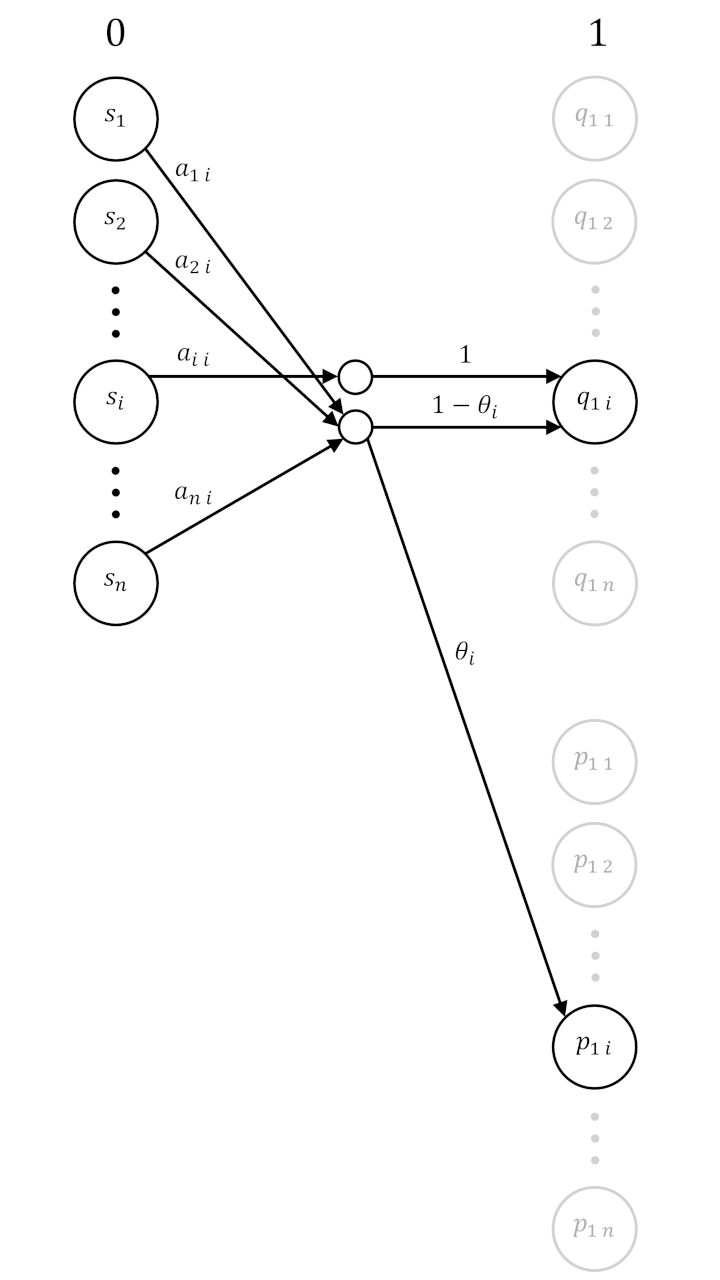
\includegraphics[width=0.7\linewidth]{figs/pq_0.png}
        \caption{$p_{t i}$と$q_{t i}$の初項, 式 (\ref{eq:q1i})を表したダイヤグラム}
        \label{fig:pqt}
    \end{center}
\end{figure}

\begin{figure}[H]
    \begin{center}
        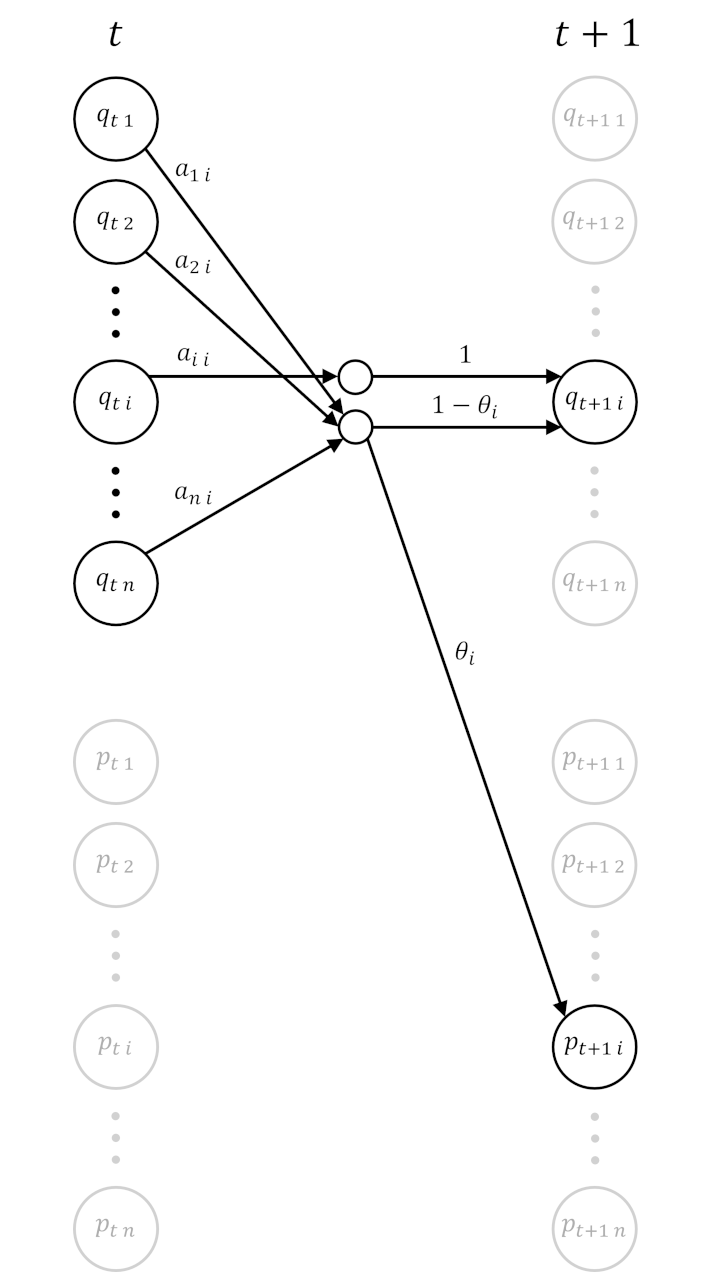
\includegraphics[width=0.7\linewidth]{figs/pq_t.png}
        \caption{$p_{t i}$と$q_{t i}$の漸化式 (\ref{eq:qti_rec}) , (\ref{eq:pti_rec}) を表したダイヤグラム}
        \label{fig:pqt}
    \end{center}
\end{figure}

次に$ p_i $について, $ \V{p} = (p_1 , p_2 , \cdots , p_n)^\mathrm{T} $とおき(\ref{eq:pt})を(\ref{eq:p_sum_pt})に代入すれば
\begin{align}
    \V{p} &= \sum_{t=1}^{\infty} \V{L} \V{K}^{t - 1} \V{s} \\
    &= \V{L} \left( \sum_{t=0}^{\infty} \V{K}^t \right) \V{s} \label{eq:p_}
\end{align}
を得る. 

ここで$ \sum \V{K}^t $が収束することを示す. 
ゲルシュゴリンの定理\cite{s_saito}より$ \V{K}^{\mathrm{T}} $の任意の固有値$ \lambda $はいずれかの$ i $に対し
\begin{equation}
    a_{i i} - \sum_{j \ne i}(1 - \theta_j) a_{i j} \le \lambda \le a_{i i} + \sum_{j \ne i}(1 - \theta_j) a_{i j}
\end{equation}
を満たす. 右の不等式についてマルコフ連鎖がエルゴード的であることから$ a_{i i} < 1 $であり, \cite{funaki}$ \theta_j > 0 $でもあるので
\begin{equation}
    \lambda < a_{i j} + \sum_{j \ne i} a_{i j} = 1
\end{equation}
となる. 同様に左の不等式についても
\begin{equation}
    \lambda > -1
\end{equation}
となる. よって$ \V{K}^\mathrm{T} $の固有値はいずれも絶対値が$ 1 $未満である. すると$ \V{K} $と$ \V{K}^{\mathrm{T}} $の固有値は等しいので$ \V{K} $の固有値も絶対値が$ 1 $未満となる. 
よって行列等比級数の公式が使えて\cite{m_saito}
\begin{equation} \label{eq:sumK}
    \sum_{t=0}^{\infty} \V{K}^t = (\V{I} - \V{K})^{-1}
\end{equation}
となる. ただし$ \V{I} $は$ n $行$ n $列の単位行列である. 

(\ref{eq:sumK})を(\ref{eq:p_})に代入すれば(\ref{eq:p})を得る. 

\section{$ \tau $が有限である確率}
下式が成り立つ. 
\begin{equation}
    \mathrm{P}(\tau < \infty) = 1
\end{equation}
これを示す. $ R_t = 0 $という事象を$ F_t $とおけば, $ \tau < \infty $という事象は$ \bigcup_{t=1}^{\infty} F_t $である. 
この事象について下の包含関係が成り立つ. 
\begin{equation} \label{eq:UFt}
    \bigcup_{t=1}^{\infty} F_t \supseteq \bigcap_{t^{\prime}=1}^{\infty} \bigcup_{t=t^{\prime}}^{\infty} F_t
\end{equation}

上式右辺の確率が1であることを示す. 
ボレル・カンテリの第二法則\cite{sato}より$ \{F_t\}_{t=1,2,\cdots} $の独立性と$ \sum_t \mathrm{P}(F_t) $が発散することを示せばよい. 
そのためにまず$ \mathrm{P}(F_t) $を求める. 
$ \mathrm{P}(F_t, M_t = m_i) $を$ r_{t i} $とおくと定義より下式が成り立つ. 
\begin{equation}\label{eq:PFt_rti}
    \mathrm{P}(F_t) = \sum_{i=1}^n r_{t i}
\end{equation}
また$ r_{t i} $は下のようになる. 
\begin{align}
    r_{t i} &= \sum_{j=1}^n \mathrm{P}(R_t = 0 , M_t = m_i , M_{t-1} = m_j) \\
    &= \sum_{j=1}^n \left(
    \begin{array}{l}
        \mathrm{P}(R_t = 0 | M_t = m_i , M_{t-1} = m_j) \\
        \times \mathrm{P}(M_t = m_i | M_{t-1} = m_j) \mathrm{P}(M_{t-1} = m_j)
    \end{array}
    \right) \label{eq:rti_P} \\
    &= \sum_{j \ne i} \theta_j a_{j i} \mathrm{P}(M_{t-1} = m_j)
\end{align}
これを$ \V{r}_t = (r_{t 1} , r_{t 2} , \cdots , r_{t n})^\mathrm{T} $とおいて行列で書けば
\begin{equation}\label{eq:rt_row}
    \V{r}_t =
    \begin{pmatrix}
        0 & \theta_1 a_{2 1} & \cdots & \theta_1 a_{n 1} \\
        \theta_2 a_{1 2} & 0 & \cdots & \theta_2 a_{n 2} \\
        \vdots & \vdots & \ddots & \vdots \\
        \theta_n a_{1 n} & \theta_n a_{2 n} & \cdots & 0 \\
    \end{pmatrix}
    \begin{pmatrix}
        \mathrm{P}(M_{t-1} = m_1) \\
        \mathrm{P}(M_{t-1} = m_2) \\
        \vdots \\
        \mathrm{P}(M_{t-1} = m_n) \\
    \end{pmatrix}
\end{equation}
となる. 右辺の係数行列は$ \V{L} $であり, ベクトルは$ i $番目の要素が$ t $回目の遷移の後動作$ m_i $である確率なので$ \V{A}^{t-1} \V{s} $である. \cite{funaki}
よって$\V{r}_t$は下のように書ける. 
\begin{equation}\label{eq:rt}
    \V{r}_t = \V{L} \V{A}^{t-1} \V{s}
\end{equation}
(\ref{eq:PFt_rti})と(\ref{eq:rt})から$ \mathrm{P}(F_t) $が求まった. 
\begin{equation} \label{eq:PFt}
    \mathrm{P}(F_t) = \V{L} \V{A}^{t-1} \V{s} \text{の全要素の和}
\end{equation}

次に$ \{F_t\}_{t=1,2,\cdots} $の独立性について, 任意の異なる$t_1, t_2 \in \{1,2,3,\cdots\}$に対し
\begin{align}
    \mathrm{P}(F_{t_1} \cap F_{t_2}) &= \mathrm{P}(F_{t_1}) \sum_{i=1}^n \mathrm{P}(F_{t_2}, M_{t_2} = m_i | F_{t_1}) \\
    &= \mathrm{P}(F_{t_1}) \sum_{i=1}^n \sum_{j=1}^n \left(
    \begin{array}{l}
        \mathrm{P}(F_{t_2} | F_{t_1}, M_{t_2} = m_i, M_{t_2 - 1} = m_j) \\
        \times \mathrm{P}(M_{t_2} = m_i | F_{t_1}, M_{t_2 - 1} = m_j) \\
        \times \mathrm{P}(M_{t_2 - 1} = m_j | F_{t_1})
    \end{array}
    \right) \\
    &= \mathrm{P}(F_{t_1}) \sum_{i=1}^n \sum_{j=1}^n \left(
    \begin{array}{l}
        \mathrm{P}(F_{t_2} | M_{t_2} = m_i, M_{t_2 - 1} = m_j) \\
        \times \mathrm{P}(M_{t_2} = m_i | M_{t_2 - 1} = m_j) \\
        \times \mathrm{P}(M_{t_2 - 1} = m_j)
    \end{array}
    \right) \label{eq:PFt1Ft2_markov} \\
    &= \mathrm{P}(F_{t_1}) \sum_{i=1}^n r_{t_2 i} \label{eq:PFt1Ft2_r}\\
    &= \mathrm{P}(F_{t_1}) \mathrm{P}(F_{t_2})
\end{align}
である. 
ただし(\ref{eq:PFt1Ft2_markov})は$ F_t $が$ M_t $と$ M_{t-1} $の組み合わせにのみ依存することと遷移のマルコフ性から, (\ref{eq:PFt1Ft2_r})は(\ref{eq:rti_P})からわかる. 
よって$ \{F_t\}_{t=1,2,\cdots} $は独立である. 

次に$ \sum_t \mathrm{P}(F_t) $が発散することを示す. 
$\V{A}^{t} \V{s} $はマルコフ連鎖のエルゴード性より$ t \to \infty $で0でないベクトルに収束する. \cite{funaki}
また$ \V{L} $はエルゴード性と遷移失敗確率$ \theta_i $が真に0より大きいことより各列に真に0より大きい成分をもつ. 
よって(\ref{eq:rt})から$ \V{r}_t $は0でないベクトルに収束し, (\ref{eq:PFt})から$ \mathrm{P}(F_t) $も真に0より大きい値に収束する. 
\begin{equation}
    \lim_{t \to \infty} \mathrm{P}(F_t) \gneq 0
\end{equation}
そのため$ \sum_t \mathrm{P}(F_t) $は無限大に発散する. 
\begin{equation}
    \sum_{t=1}^{\infty} \mathrm{P}(F_t) = \infty
\end{equation}

ここまでで下式が示された. 
\begin{equation} \label{eq:PlimsupFt}
    \mathrm{P}\left( \bigcap_{t^{\prime}=1}^{\infty} \bigcup_{t=t^{\prime}}^{\infty} F_t \right) = 1
\end{equation}
この式と(\ref{eq:UFt})より
\begin{align}
    \mathrm{P}\left( \bigcup_{t=1}^{\infty} F_t \right) &\ge \mathrm{P}\left( \bigcap_{t^{\prime}=1}^{\infty} \bigcup_{t=t^{\prime}}^{\infty} F_t \right)\\
    &= 1
\end{align}
なので下式が成り立つ. 
\begin{equation}
    \mathrm{P}\left(\bigcup_{t=1}^{\infty} F_t \right) = 1
\end{equation}
以上より$ \tau $が有限である確率は$ 1 $である. 

またこのことからなくしもの位置分布$ h $について下式が成り立つ. 
\begin{equation}
    \int_X h \mathrm{d}x = 1
\end{equation}
上式は定義$ h = \sum_i p_i b_i $, $ \int_X b_i = 1 $と下式よりわかる. 
\begin{align}
    \sum_{i=1}^n p_i &= \mathrm{P}(\tau < \infty) \\
    &= 1
\end{align}
